\documentclass{article}
\usepackage{tikz,xcolor}
\usetikzlibrary{intersections}
\begin{document}
\tableofcontents
\section{Setting up the Environment in \LaTeX{}}
\begin{tikzpicture}
\draw (-1.5,0) -- (1.5,0);
\draw (0,-1.5) -- (0,1.5);
\end{tikzpicture}

\section{Curved Path Construction}
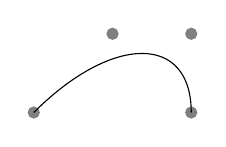
\begin{tikzpicture}
\filldraw [gray] (0,0) circle [radius=2pt]
(1,1) circle [radius=2pt]
(2,1) circle [radius=2pt]
(2,0) circle [radius=2pt];
\draw (0,0) .. controls (1,1) and (2,1) .. (2,0);
\end{tikzpicture}

\begin{tikzpicture}
\draw (-1.5,0) -- (1.5,0);
\draw (0,-1.5) -- (0,1.5);
\draw (-1,0) .. controls (-1,0.555) and (-0.555,1) .. (0,1)
.. controls (0.555,1) and (1,0.555) .. (1,0);
\end{tikzpicture}

\section{Circle Path Construction}
\tikz \draw (0,0) circle [radius=10pt];
\tikz \draw (0,0) ellipse [x radius=20pt, y radius=10pt];
\begin{tikzpicture}
\draw (-1.5,0) -- (1.5,0);
\draw (0,-1.5) -- (0,1.5);
\draw (0,0) circle [radius=1cm];
\end{tikzpicture}

\section{Rectangle Path Construction}
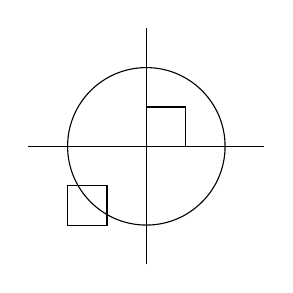
\begin{tikzpicture}
\draw (-1.5,0) -- (1.5,0);
\draw (0,-1.5) -- (0,1.5);
\draw (0,0) circle [radius=1cm];
\draw (0,0) rectangle (0.5,0.5);
\draw (-0.5,-0.5) rectangle (-1,-1);
\end{tikzpicture}

\section{Grid Path Construction}
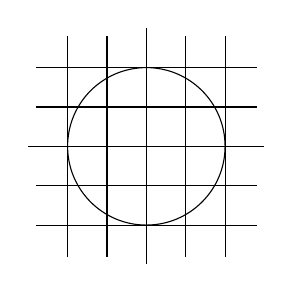
\begin{tikzpicture}
\draw (-1.5,0) -- (1.5,0);
\draw (0,-1.5) -- (0,1.5);
\draw (0,0) circle [radius=1cm];
\draw[step=.5cm] (-1.4,-1.4) grid (1.4,1.4);
\end{tikzpicture}

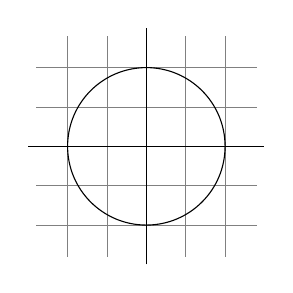
\begin{tikzpicture}
\draw[step=.5cm,gray,very thin] (-1.4,-1.4) grid (1.4,1.4);
\draw (-1.5,0) -- (1.5,0);
\draw (0,-1.5) -- (0,1.5);
\draw (0,0) circle [radius=1cm];
\end{tikzpicture}

\section{Adding a Touch of Style}
\begin{tikzpicture}
[Karl's grid/.style ={help lines,color=#1!50},
Karl's grid/.default=blue]
\draw[Karl's grid] (0,0) grid (1.5,2);
\draw[Karl's grid=red] (2,0) grid (3.5,2);
\end{tikzpicture}

\section{Arc Path Construction}
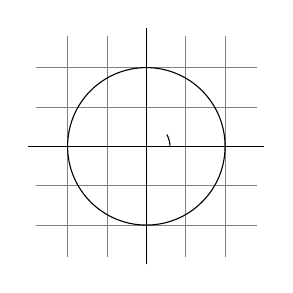
\begin{tikzpicture}
\draw[step=.5cm,gray,very thin] (-1.4,-1.4) grid (1.4,1.4);
\draw (-1.5,0) -- (1.5,0);
\draw (0,-1.5) -- (0,1.5);
\draw (0,0) circle [radius=1cm];
\draw (3mm,0mm) arc [start angle=0, end angle=30, radius=3mm];
\end{tikzpicture}
\begin{tikzpicture}[scale=3]
\draw[step=.5cm,gray,very thin] (-1.4,-1.4) grid (1.4,1.4);
\draw (-1.5,0) -- (1.5,0);
\draw (0,-1.5) -- (0,1.5);
\draw (0,0) circle [radius=1cm];
\draw (3mm,0mm) arc [start angle=0, end angle=30, radius=3mm];
\end{tikzpicture}

%%??
\begin{tikzpicture}[scale=3]
\draw[step=.5cm,gray,very thin] (-1.4,-1.4) grid (1.4,1.4);
\draw (-1.5,0) -- (1.5,0);
\draw (0,-1.5) -- (0,1.5);
\draw (0,0) circle [radius=1cm];
\draw (3mm,0mm) arc [start angle=20, end angle=30, radius=3mm];
\end{tikzpicture}

\tikz \draw (0,0)
arc [start angle=0, end angle=315,
x radius=1.75cm, y radius=1cm];

\section{Clipping a Path}
% You can use the \clip command to clip all subsequent drawing. It works like \draw, only it does not draw anything, but uses the given path to clip everything subsequently.
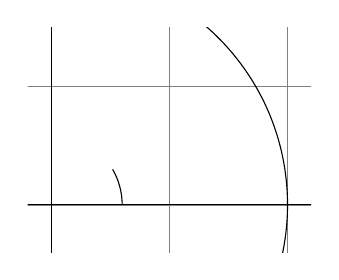
\begin{tikzpicture}[scale=3]
\clip (-0.1,-0.2) rectangle (1.1,0.75);
\draw[step=.5cm,gray,very thin] (-1.4,-1.4) grid (1.4,1.4);
\draw (-1.5,0) -- (1.5,0);
\draw (0,-1.5) -- (0,1.5);
\draw (0,0) circle [radius=1cm];
\draw (3mm,0mm) arc [start angle=0, end angle=30, radius=3mm];
\end{tikzpicture}

% You can also do both at the same time: Draw and clip a path.
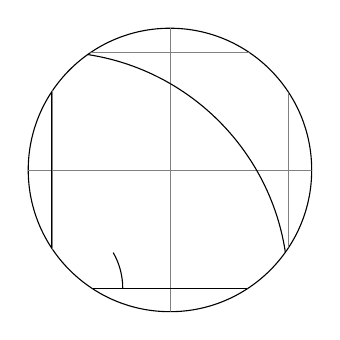
\begin{tikzpicture}[scale=3]
\clip[draw] (0.5,0.5) circle (.6cm);
\draw[step=.5cm,gray,very thin] (-1.4,-1.4) grid (1.4,1.4);
\draw (-1.5,0) -- (1.5,0);
\draw (0,-1.5) -- (0,1.5);
\draw (0,0) circle [radius=1cm];
\draw (3mm,0mm) arc [start angle=0, end angle=30, radius=3mm];
\end{tikzpicture}

% clip without draw
\begin{tikzpicture}[scale=3]
\clip (0.5,0.5) circle (.6cm);
\draw[step=.5cm,gray,very thin] (-1.4,-1.4) grid (1.4,1.4);
\draw (-1.5,0) -- (1.5,0);
\draw (0,-1.5) -- (0,1.5);
\draw (0,0) circle [radius=1cm];
\draw (3mm,0mm) arc [start angle=0, end angle=30, radius=3mm];
\end{tikzpicture}

\section{Parabola and Sine Path Construction}
\tikz \draw (0,0) rectangle (1,1) (0,0) parabola (1,1);
\tikz \draw[x=1pt,y=1pt] (0,0) parabola bend (4,16) (6,12);
A sine \tikz \draw[x=1ex,y=1ex] (0,0) sin (1.57,1); curve.
\tikz \draw[x=1.57ex,y=1ex] (0,0) sin (1,1) cos (2,0) sin (3,-1) cos (4,0)
(0,1) cos (1,0) sin (2,-1) cos (3,0) sin (4,1);

\section{Filling and Drawing}
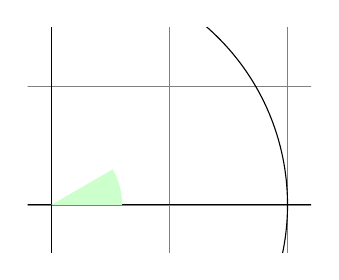
\begin{tikzpicture}[scale=3]
\clip (-0.1,-0.2) rectangle (1.1,0.75);
\draw[step=.5cm,gray,very thin] (-1.4,-1.4) grid (1.4,1.4);
\draw (-1.5,0) -- (1.5,0);
\draw (0,-1.5) -- (0,1.5);
\draw (0,0) circle [radius=1cm];
\fill[green!20!white] (0,0) -- (3mm,0mm)
arc [start angle=0, end angle=30, radius=3mm] -- (0,0);
\end{tikzpicture}

%\fill[green!20!white] (0,0) -- (3mm,0mm) arc [start angle=0, end angle=30, radius=3mm] -- cycle;

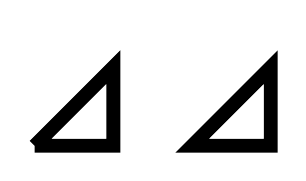
\begin{tikzpicture}[line width=5pt]
\draw (0,0) -- (1,0) -- (1,1) -- (0,0);
\draw (2,0) -- (3,0) -- (3,1) -- cycle;
\useasboundingbox (0,1.5); % make bounding box higher
\end{tikzpicture}

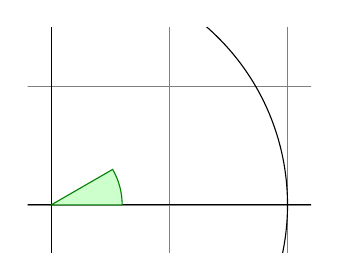
\begin{tikzpicture}[scale=3]
\clip (-0.1,-0.2) rectangle (1.1,0.75);
\draw[step=.5cm,gray,very thin] (-1.4,-1.4) grid (1.4,1.4);
\draw (-1.5,0) -- (1.5,0);
\draw (0,-1.5) -- (0,1.5);
\draw (0,0) circle [radius=1cm];
\filldraw[fill=green!20!white, draw=green!50!black] (0,0) -- (3mm,0mm)
arc [start angle=0, end angle=30, radius=3mm] -- cycle;
\end{tikzpicture}

\section{Shading}
\tikz \shade (0,0) rectangle (2,1) (3,0.5) circle (.5cm);

\begin{tikzpicture}[rounded corners,ultra thick]
\shade[top color=yellow,bottom color=black] (0,0) rectangle +(2,1);
\shade[left color=yellow,right color=black] (3,0) rectangle +(2,1);
\shadedraw[inner color=yellow,outer color=black,draw=yellow] (6,0) rectangle +(2,1);
\shade[ball color=green] (9,.5) circle (.5cm);
\end{tikzpicture}

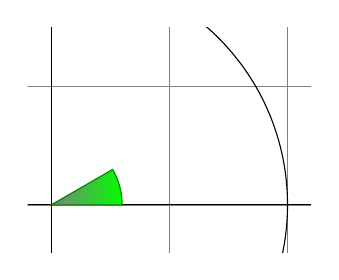
\begin{tikzpicture}[scale=3]
\clip (-0.1,-0.2) rectangle (1.1,0.75);
\draw[step=.5cm,gray,very thin] (-1.4,-1.4) grid (1.4,1.4);
\draw (-1.5,0) -- (1.5,0);
\draw (0,-1.5) -- (0,1.5);
\draw (0,0) circle [radius=1cm];
\shadedraw[left color=gray,right color=green, draw=green!50!black]
(0,0) -- (3mm,0mm)
arc [start angle=0, end angle=30, radius=3mm] -- cycle;
\end{tikzpicture}

\section{Specifying Coordinates}
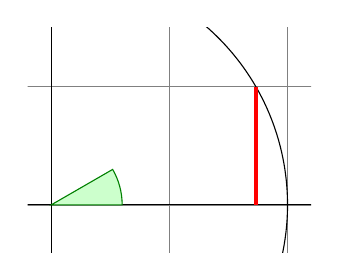
\begin{tikzpicture}[scale=3]
\clip (-0.1,-0.2) rectangle (1.1,0.75);
\draw[step=.5cm,gray,very thin] (-1.4,-1.4) grid (1.4,1.4);
\draw (-1.5,0) -- (1.5,0);
\draw (0,-1.5) -- (0,1.5);
\draw (0,0) circle [radius=1cm];
\filldraw[fill=green!20,draw=green!50!black] (0,0) -- (3mm,0mm)
arc [start angle=0, end angle=30, radius=3mm] -- cycle;
\draw[red,very thick] (30:1cm) -- +(0,-0.5);
\end{tikzpicture}


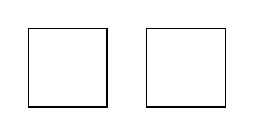
\begin{tikzpicture}
\def\rectanglepath{-- ++(1cm,0cm) -- ++(0cm,1cm) -- ++(-1cm,0cm) -- cycle}
\draw (0,0) \rectanglepath;
\draw (1.5,0) \rectanglepath;
\end{tikzpicture}

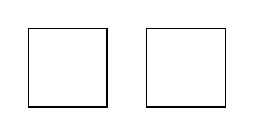
\begin{tikzpicture}
\def\rectanglepath{-- +(1cm,0cm) -- +(1cm,1cm) -- +(0cm,1cm) -- cycle}
\draw (0,0) \rectanglepath;
\draw (1.5,0) \rectanglepath;
\end{tikzpicture}

\tikz \draw (0,0) rectangle +(1,1) (1.5,0) rectangle +(1,1);

\section{Intersecting Paths}
\begin{tikzpicture}
\path [name path=upward line] (1,0) -- (1,1);
\path [name path=sloped line] (0,0) -- (30:1.5cm); % a bit longer, so that there is an intersection
% (add `\usetikzlibrary{intersections}' after loading tikz in the preamble)
\draw [name intersections={of=upward line and sloped line, by=x}]
[very thick,orange] (1,0) -- (x);
\end{tikzpicture}

\section{Adding Arrow Tips}
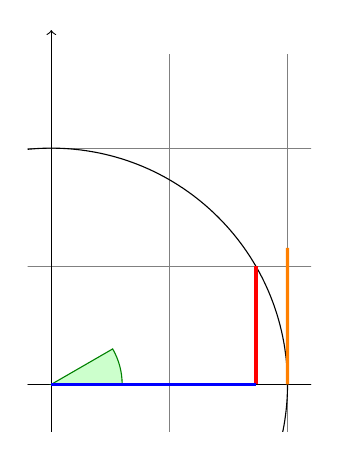
\begin{tikzpicture}[scale=3]
\clip (-0.1,-0.2) rectangle (1.1,1.51);
\draw[step=.5cm,gray,very thin] (-1.4,-1.4) grid (1.4,1.4);
\draw[->] (-1.5,0) -- (1.5,0);
\draw[->] (0,-1.5) -- (0,1.5);
\draw (0,0) circle [radius=1cm];
\filldraw[fill=green!20,draw=green!50!black] (0,0) -- (3mm,0mm)
arc [start angle=0, end angle=30, radius=3mm] -- cycle;
\draw[red,very thick] (30:1cm) -- +(0,-0.5);
\draw[blue,very thick] (30:1cm) ++(0,-0.5) -- (0,0);
\path [name path=upward line] (1,0) -- (1,1);
\path [name path=sloped line] (0,0) -- (30:1.5cm);
\draw [name intersections={of=upward line and sloped line, by=x}]
[very thick,orange] (1,0) -- (x);
\end{tikzpicture}

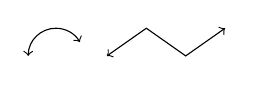
\begin{tikzpicture}
\draw [<->] (0,0) arc [start angle=180, end angle=30, radius=10pt];
\draw [<->] (1,0) -- (1.5cm,10pt) -- (2cm,0pt) -- (2.5cm,10pt);
\end{tikzpicture}

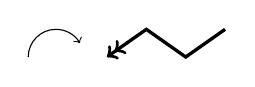
\begin{tikzpicture}
\draw [->] (0,0) arc [start angle=180, end angle=30, radius=10pt];
\draw [<<-,very thick] (1,0) -- (1.5cm,10pt) -- (2cm,0pt) -- (2.5cm,10pt);
\end{tikzpicture}

\section{Scoping}
\begin{tikzpicture}[ultra thick]
\draw (0,0) -- (0,1);
\begin{scope}[thin]
\draw (1,0) -- (1,1);
\draw (2,0) -- (2,1);
\end{scope}
\draw (3,0) -- (3,1);
\end{tikzpicture}

\section{Transformations}
\tikz \draw (0,0) -- (0,0.5) [xshift=2pt] (0,0) -- (0,0.5);
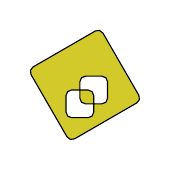
\begin{tikzpicture}[even odd rule,rounded corners=2pt,x=10pt,y=10pt]
\filldraw[fill=yellow!80!black] (0,0) rectangle (1,1)
[xshift=5pt,yshift=5pt] (0,0) rectangle (1,1)
[rotate=30] (-1,-1) rectangle (2,2);
\end{tikzpicture}

\section{Repeating Things: For-Loops}
\foreach \x in {1,2,3} {$x =\x$, }

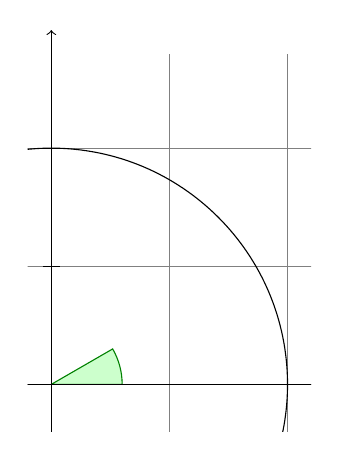
\begin{tikzpicture}[scale=3]
\clip (-0.1,-0.2) rectangle (1.1,1.51);
\draw[step=.5cm,gray,very thin] (-1.4,-1.4) grid (1.4,1.4);
\filldraw[fill=green!20,draw=green!50!black] (0,0) -- (3mm,0mm)
arc [start angle=0, end angle=30, radius=3mm] -- cycle;
\draw[->] (-1.5,0) -- (1.5,0);
\draw[->] (0,-1.5) -- (0,1.5);
\draw (0,0) circle [radius=1cm];
\foreach \x in {-1cm,-0.5cm,1cm}
\draw (\x,-1pt) -- (\x,1pt);
\foreach \y in {-1cm,-0.5cm,0.5cm,1cm}
\draw (-1pt,\y) -- (1pt,\y);
\end{tikzpicture}

\tikz\foreach \x in {-1,-0.5,1}
\draw[xshift=\x cm] (0pt,-1pt) -- (0pt,1pt);

\tikz \foreach \x in {1,...,10}
\draw (\x,0) circle (0.4cm);

\tikz \foreach \x in {-1,-0.5,...,1}
\draw (\x cm,-1pt) -- (\x cm,1pt);

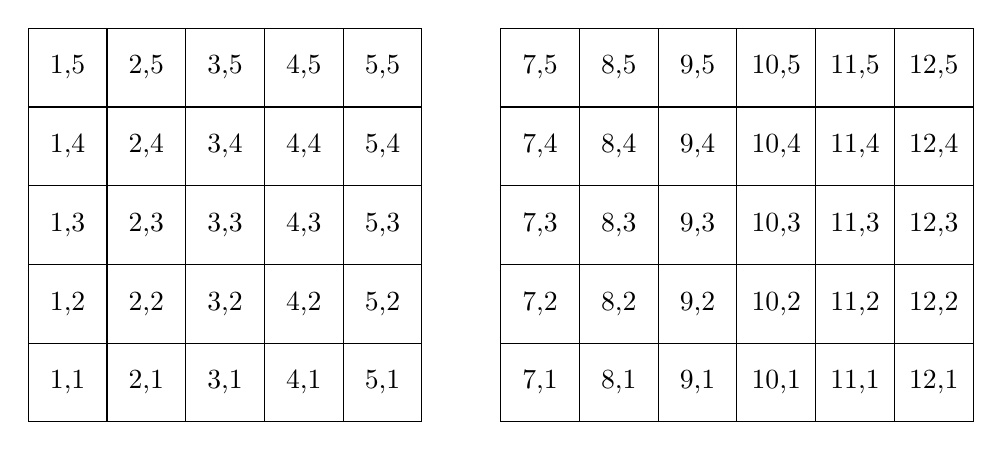
\begin{tikzpicture}
\foreach \x in {1,2,...,5,7,8,...,12}
\foreach \y in {1,...,5}
{
\draw (\x,\y) +(-.5,-.5) rectangle ++(.5,.5);
\draw (\x,\y) node{\x,\y};
}
\end{tikzpicture}

\section{Adding Text}
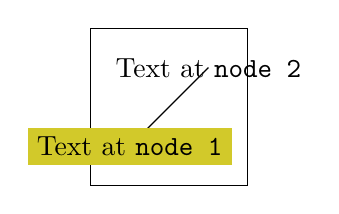
\begin{tikzpicture}
\draw (0,0) rectangle (2,2);
\draw (0.5,0.5) node [fill=yellow!80!black]
{Text at \verb!node 1!}
-- (1.5,1.5) node {Text at \verb!node 2!};
\end{tikzpicture}
\end{document}
